\begin{IEEEbiography}[{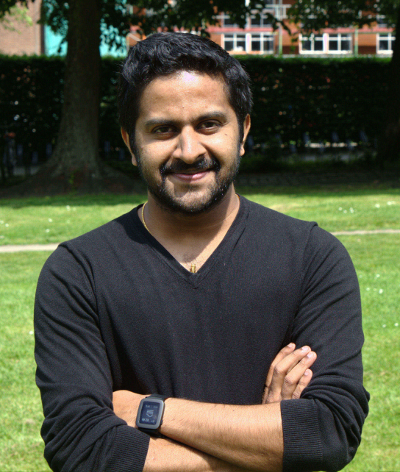
\includegraphics[width=1in,height=1.25in,clip,keepaspectratio]{figures/sreeraj}}]
    {Sreeraj Rajendran}
received his Masters degree in communication and signal processing from the Indian Institute of Technology, Bombay, in 2013. He is currently pursuing the PhD degree in the Department of Electrical Engineering, KU Leuven, Belgium. Before joining KU Leuven, he worked as a senior design engineer in the baseband team of Cadence and as an ASIC verification engineer in Wipro Technologies. His main research interests include machine learning algorithms for wireless and low power wireless sensor networks.
\end{IEEEbiography}


\begin{IEEEbiography}[{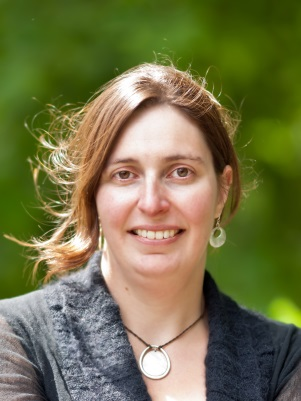
\includegraphics[width=1in,height=1.25in,clip,keepaspectratio]{figures/sofie}}]
    {Sofie Pollin}
obtained her PhD degree at KU Leuven with honors in 2006. From 2006-2008 she continued her research on wireless communication, energy-efficient networks, cross-layer design, coexistence and cognitive radio at UC Berkeley.  In November 2008 she returned to imec to become a principal scientist in the green radio team. Since 2012, she is tenure track assistant professor at the electrical engineering department at KU Leuven. Her research centers around Networked Systems that require networks that are ever more dense, heterogeneous, battery powered and spectrum constrained. Prof. Pollin is BAEF and Marie Curie fellow, and IEEE senior member. 
\end{IEEEbiography}